% Two kinds of discrepancy, distinguished by where they enter.
%   top    -- beta is a species-level bias, upstream of h_r, so it propagates
%             through the composition (a ratio inherits a difference).
%   bottom -- gamma and kappa act on the finished row, downstream of h_r, and
%             pivot about the study's own level c_rc.
%
%   compile:  pdflatex discrepancy.tex
%
\documentclass[border=10pt]{standalone}
\usepackage{lmodern}
\usepackage{amsmath}
\usepackage{amssymb}
\usepackage{tikz}
\usetikzlibrary{arrows.meta,positioning,calc,decorations.pathreplacing}
% Shared palette for the population-model figures.
%   ink      body / structure
%   popcol   the patient cloud and anything predicted from it
%   mechcol  the simulator and species-level quantities
%   msrcol   the measurement map (readout-level: gamma, kappa)
%   datacol  reported rows
\definecolor{ink}{HTML}{3A3A3A}
\definecolor{popcol}{HTML}{3B4AA6}
\definecolor{mechcol}{HTML}{2E7D5B}
\definecolor{msrcol}{HTML}{EB811B}
\definecolor{datacol}{HTML}{8C3B4A}


\begin{document}
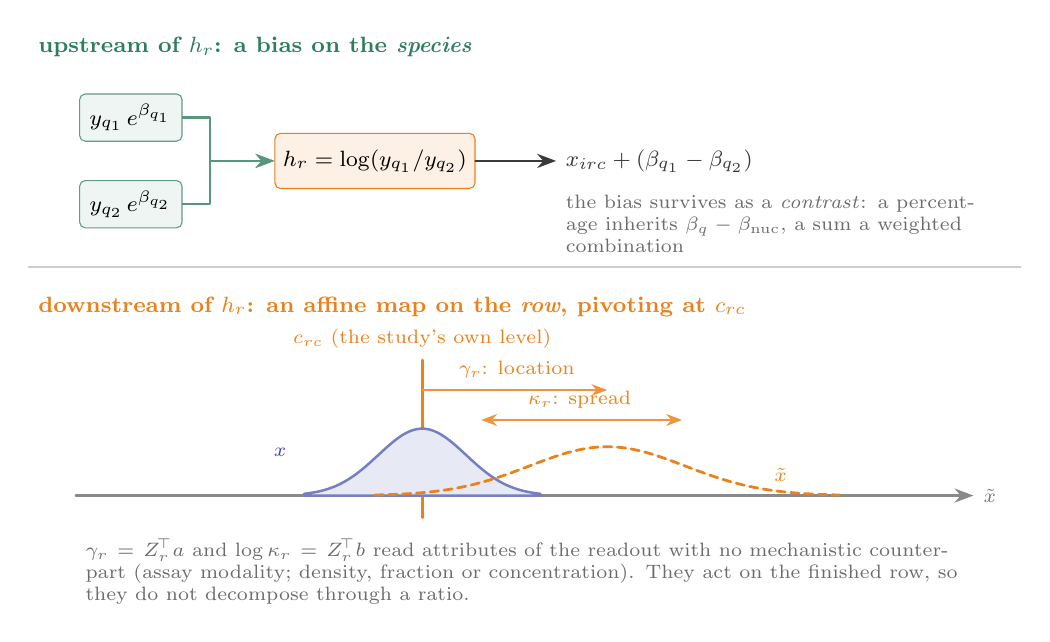
\begin{tikzpicture}[
  font=\sffamily, >=Stealth, line cap=round, line join=round,
  sp/.style={draw=mechcol!75, fill=mechcol!8, rounded corners=2pt,
             minimum width=13mm, minimum height=6mm, inner sep=1.5pt,
             font=\footnotesize},
  op/.style={draw=msrcol, fill=msrcol!12, rounded corners=2pt,
             minimum height=7mm, inner sep=3pt, font=\footnotesize},
  fl/.style={-{Stealth[length=2.4mm]}, ink, line width=0.85pt}]

% ================================================================ upstream
\node[font=\footnotesize\bfseries, mechcol, anchor=west] at (-0.4,2.35)
  {upstream of $h_r$: a bias on the \emph{species}};

\node[sp] (y1) at (0.9,1.45) {$y_{q_1}\,e^{\beta_{q_1}}$};
\node[sp] (y2) at (0.9,0.35) {$y_{q_2}\,e^{\beta_{q_2}}$};

\node[op] (hr) at (4.0,0.90) {$h_r=\log(y_{q_1}/y_{q_2})$};
\draw[fl,mechcol!80] (y1.east) -- ++(0.35,0) |- (hr.west);
\draw[fl,mechcol!80] (y2.east) -- ++(0.35,0) |- (hr.west);

\node[anchor=west, font=\footnotesize, ink] (out) at (6.3,0.90)
  {$x_{irc}+(\beta_{q_1}-\beta_{q_2})$};
\draw[fl] (hr.east) -- (out.west);

\node[anchor=west, font=\scriptsize, ink!75, align=left, text width=52mm] at (6.3,0.10)
  {the bias survives as a \emph{contrast}: a percentage inherits
   $\beta_q-\beta_{\mathrm{nuc}}$, a sum a weighted combination};

\draw[ink!25, line width=0.6pt] (-0.4,-0.45) -- (12.2,-0.45);

% ================================================================ downstream
\node[font=\footnotesize\bfseries, msrcol, anchor=west] at (-0.4,-0.95)
  {downstream of $h_r$: an affine map on the \emph{row}, pivoting at $c_{rc}$};

\begin{scope}[shift={(0,-3.35)}]
  % axis
  \draw[ink!60, line width=0.8pt, -{Stealth[length=2.4mm]}] (0.2,0) -- (11.6,0)
    node[right, font=\scriptsize, ink!70] {$\tilde x$};
  % pivot
  \draw[msrcol, line width=1pt] (4.6,-0.28) -- (4.6,1.72);
  \node[msrcol, font=\scriptsize, anchor=south] at (4.6,1.74) {$c_{rc}$ (the study's own level)};

  % predicted spread, before the map
  \draw[popcol!70, fill=popcol!12, line width=0.9pt]
    plot[domain=3.1:6.1,samples=70,smooth] (\x,{0.85*exp(-(\x-4.6)*(\x-4.6)/0.62)})
    -- (6.1,0) -- (3.1,0) -- cycle;
  % after kappa (stretched about the pivot) and gamma (shifted right)
  \draw[msrcol, densely dashed, line width=1pt]
    plot[domain=4.0:9.9,samples=90,smooth] (\x,{0.62*exp(-(\x-6.95)*(\x-6.95)/1.95)});

  % gamma: shift
  \draw[msrcol!85, -{Stealth[length=2mm]}, line width=0.8pt] (4.6,1.34) -- (6.95,1.34);
  \node[msrcol, font=\scriptsize, anchor=south] at (5.8,1.36) {$\gamma_r$: location};
  % kappa: stretch about the pivot
  \draw[msrcol!85, {Stealth[length=2mm]}-{Stealth[length=2mm]}, line width=0.8pt]
    (5.35,0.96) -- (7.9,0.96);
  \node[msrcol, font=\scriptsize, anchor=south] at (6.6,0.98) {$\kappa_r$: spread};

  \node[popcol, font=\scriptsize, anchor=east] at (3.0,0.55) {$x$};
  \node[msrcol, font=\scriptsize, anchor=west] at (8.95,0.26) {$\tilde x$};

  \node[anchor=north west, font=\scriptsize, ink!75, align=left, text width=112mm] at (0.2,-0.42)
    {$\gamma_r=Z_r^{\!\top}a$ and $\log\kappa_r=Z_r^{\!\top}b$ read attributes of the readout with no
     mechanistic counterpart (assay modality; density, fraction or concentration).
     They act on the finished row, so they do not decompose through a ratio.};
\end{scope}

\end{tikzpicture}
\end{document}
